\documentclass[10pt,a4paper]{article}
\usepackage[margin=17mm]{geometry}
\usepackage{graphicx}
\usepackage{booktabs}
\usepackage{microtype}
\usepackage[T1]{fontenc}
\usepackage{lmodern}
\setlength{\parindent}{0pt}
\setlength{\parskip}{5pt}
\begin{document}
\begin{center}
{\Large Recovered original paired Kummer run}\\[3pt]
{\small run-20261022T0710Z \quad retrospective report, 2026-10-22 UTC}
\end{center}

\textbf{Provenance.} The migrated source transcript pins the original
\texttt{paired\_uncached} command, working directory, exit status and combined
output. Its SHA-256 and exact event coordinates are in the study's recovered
execution receipt. A locked offline build
at the saved source path reproduced the retained executable byte for byte.

\begin{center}
\begin{tabular}{ll}
\toprule
Recorded property & Value \\
\midrule
Derived start, UTC & 07:10:45.527 \\
Completion, UTC & 07:35:52.725 \\
Elapsed process duration & 1,507.197243106 s \\
Exit code & 0 \\
Candidate results & 1,260 solved / 1,260 requested \\
Same-process rho results & 1,260 / 1,260 \\
\bottomrule
\end{tabular}
\end{center}

\textbf{Evidence boundary.} The original run did not retain separate stdout
and stderr, a standalone environment snapshot, user/system CPU time, or an
isolation level. Its elapsed duration is not a qualified wall-speed
measurement. The archived seven candidate and seven rho JSONL files are
bound by the study SHA-256 manifest. The independent Rust analyzer verifies
source scalars and recomputes its five analysis files and validation gate.
A later isolated full replay with separate process capture produced identical
raw and analysis bytes.

\textbf{Modeled result.} Across 36 whole-cohort price cells, the full-cold
candidate/rho operation-cost ratio is 8.959687--55.935424, with zero pooled
candidate wins. At $S/M=0.5$, $I/M=10$ and 0.1 GAE per native logical
operation, it is 14.356662. These are model ratios, not wall-time ratios.
The price graph on page 2 is from the sealed study SVG and a 150 dpi render.
A later Lean theorem proves only a conditional aggregation step on aligned
natural-number price vectors; it does not import this CSV or prove the
Kummer formulas.

\textbf{Reproduction and limits.} The adjacent \texttt{RUN.md} links exact
source paths, raw records, validation, the independent analyzer and the
fresh validation replay. The conclusion is restricted to 1,260 public
workloads and the recorded GAE price model. No practical-size attack is
established.

\clearpage
\begin{center}
{\large Archived same-process price graph}\par
{\small 1,260 public targets; 36 whole-cohort price cells; modeled GAE units}
\end{center}
\vspace{8mm}
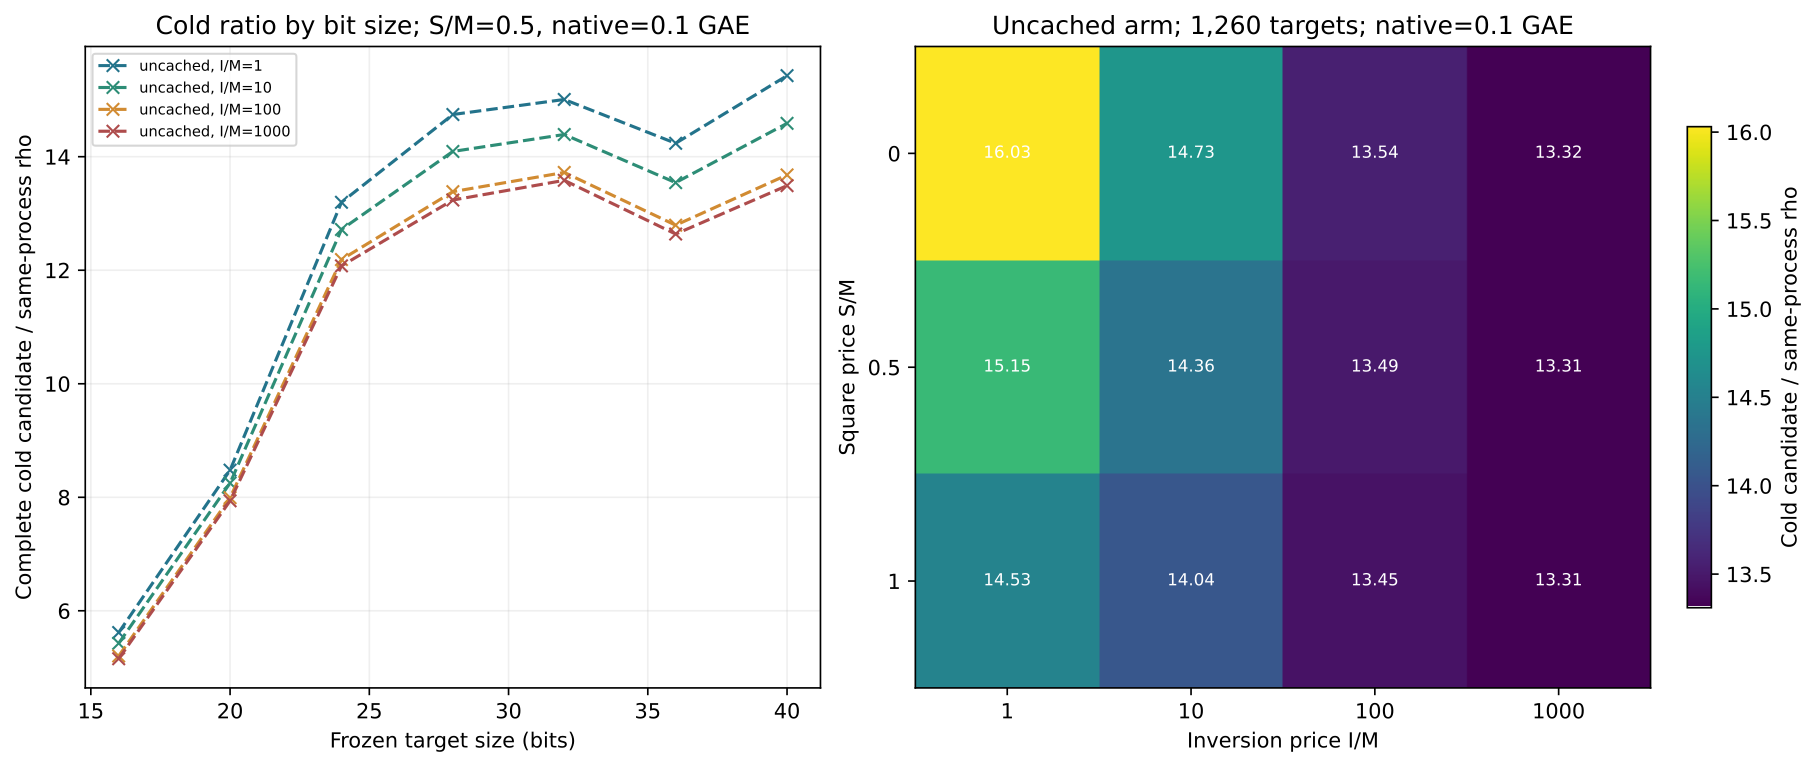
\includegraphics[width=\textwidth]{collector-cost-paired.png}
\vspace{4mm}

The full-cold candidate charge includes fresh model, theta and torsion
setup per target, source transfer, signed anchor, collector and
verification. The rho control is the native negation solver run after the
candidate in the same executable on the same workload IDs.
\end{document}
